%!TEX = xelatex
\documentclass[conference]{IEEEtran}
\IEEEoverridecommandlockouts
\usepackage[style=ieee]{biblatex}
    \addbibresource{references.bib}
\usepackage{graphicx}
\usepackage{amsmath}
\usepackage{amssymb}
\usepackage{xcolor}
    \newcommand{\todo}[1]{\textcolor{red}{[ #1 ]}}
    \newcommand{\instruction}[1]{\textcolor{orange}{#1}}
    \renewcommand{\todo}[1]{} % Uncomment to hide todos.
    \renewcommand{\instruction}[1]{} % Uncomment to hide instructions.

\newcommand{\hidden}[1]{}

\usepackage[colorlinks=false]{hyperref}

\title{STATS 402 - Interdisciplinary Data Analysis\\
    Resource-Constrained Deep Reinforcement Learning for Battlesnake\\
    Milestone Report: Stage 3
}
\author{\IEEEauthorblockN{Steven Hé (Sīchàng)\\
    sichang.he@dukekunshan.edu.cn
}}

\begin{document}
\maketitle

\begin{abstract}
    We outlines our efforts to optimize and enhance the performance of our
    reinforcement learning agents in the Battlesnake game environment.
    We delve into various aspects of customization,
    including training loop modifications and exploration of neural network
    architectures for feature extraction. Additionally,
    we discuss critical modifications to the training setup aimed at improving
    model convergence and effectiveness. Despite our rigorous efforts,
    challenges such as strategy collapse and inefficient exploration persist.
    To overcome these obstacles,
    we propose to integrate model predictions with tree search techniques.
    By detailing our plans for further experimentation and development,
    we aim to advance the competitiveness of our agents,
    and test it in the real-world among the Battlesnake community.
\end{abstract}

\instruction{
    There are no specific requirements for the stage 3 report since the progress
    may vary among different groups. Generally,
    there are four parts you need to cover in your report.
}

\section{Current Status}

\todo{
    For example, the detailed techniques you adopted to conduct the project.
    Has your group made any technical route adjustments?
    This part is essential for the groups whose actual adopted method is
    different from their milestone report 1 and report 2.
    You need to explain the reason for the change.
}

\subsection{Training Customization}

We directly customized the training loop in Stable
Baselines3~\cite{raffin2024stable}
to simplify the logic and prepare for the implementation to train the agent
against older versions of itself for 20\% of the time.
Because Battlesnake is a multi-player simultaneous-move game,
and Stable Baselines3 only supports single-agent environments,
previously, we created our environment
following the Pettingzoo~\cite{terry2021pettingzoo} parallel environment API,
and used SuperSuit~\cite{SuperSuit} to wrap it.

However, using SuperSuit for wrapping introduces two major downsides. First,
complexity is massively increased,
as SuperSuit requires multiple layers of wrappers.
This obstructs the understanding of the training process and hinders any
modifications to it, such as the old-version self-training. Second,
SuperSuit produces empty observations and zero rewards for dead agents,
so they appear alive,
and the environment appears to be a Stable Baselines3 vectorized environment.
These useless padding not only wastes computation during training,
but raises uncertainty.
Since dead agents' actions are counted into the number of steps the model has
trained, it is unclear how many steps the model has actually trained.
Additionally, it is unclear how the padding affects the training.

We modified and overrode the training methods on Stable Baselines3's PPO
implementation. Our implementation tracks each agent's statistics separately,
and only pushes them to calculate the returns and advantages when the agent
dies. We also correctly count the number of steps the model has trained,
by summing the number of steps each alive agent moves.
Although our implementation is not vectorized,
it still uses all available CPU cores on our server with dual EPYC 7763 64-Core
processors. Training for $16^5$ steps took 3777 seconds,
longer than the 3060 seconds the previous implementation took. However,
we note that the previous training was counting padding steps,
meaning that the new implementation has effectively trained more steps.

\subsection{Neural Network Architectures Exploration for Feature Extraction}

Following our plan,
we constructed more complex and larger neural networks to better extract
features from the game board. The main models include a VGG-like model,
a deeper MLP model, and small and big Vision Transformer (ViT) models.

\paragraph{VGG-like Model}
We constructed convolutional neural network (CNN) layers for feature extraction,
referencing the VGG16 model~\cite{simonyan2014very}.
Our feature layers consist of the first 7 convolutional layers,
the first 3 max-pooling layers, and the adaptive average layer in VGG16,
incrementally compressing the input feature matrices from $\mathbb R^{9\times
            21\times 21}$ to $\mathbb R^{256\times 2\times 2}$.
The features are then flattened and fed into 3-layer MLPs with hidden layer
widths 256 for either policy or value networks.
Our implementation references the PyTorch~\cite{paszke2019pytorch}
VGG16 model implementation.

We constructed a shallower and thinner model than the VGG16 model primarily for
two reasons: our feature matrices are smaller,
and our compute resources are limited.
We only used the first 3 max-pooling layers because our feature matrices have
width 21 instead of the 224 in VGG16. That is,
after all 5 max-pooling layers with kernel size 2 in VGG16,
the feature matrices would be compressed from width 224 to 7; in comparison,
our feature matrices are compressed from width 21 to 2 after 3 similar
max-pooling layers.
Additionally, we believe that the game board of Battlesnake is simple enough,
that $256\times 2\times 2=1024$ numbers are sufficient to extract the features,
and MLP layers with width 256 are sufficient to learn these smaller features.

After initial testing, the VGG-like model performed poorly,
therefore we added a residual layer to it.
Our reasoning is the CNN layers may lose the positional information,
e.g., the snake's head is always at the center of the feature matrices;
also, the network's larger depth might result in the vanishing gradient problem.
The residual is a 2-layer MLP with hidden layer of width 2048,
transforming the input features from $\mathbb R^{9\times 21\times 21}$ to
$\mathbb R^{1024}$ before adding them to the output of the CNN layers.

\paragraph{Deeper MLP Model}
Besides the VGG-like model,
we also constructed a deeper MLP model to test the performance of simple
feed-forward neural networks.
Our deeper MLP consists of a feature extractor with 4 hidden layers of width
1024 and a residual layer,
as well as separate 3-layer MLPs for either policy and value network,
with hidden layer width 512 and 256.

\paragraph{Vision Transformer (ViT) Models}
Since the ViT model has shown great success in image classification tasks as an
alternative to CNN models,
we constructed small and big ViT models for feature extraction.
Our small ViT has patch size 7, 4 encoder layers, 4 heads, hidden size 256,
and MLP size 512.
It is modified to override the convolutional kernel to have input channel size 9
instead of 3,
because our feature matrices have 9 channels instead of the 3 used in image
classification.

\subsection{Training Setup Modifications}

We realized the default entropy coefficient of 0 in the Stable Baselines3
implementation has been used,
causing insufficient exploration and convergence to spinning. Therefore,
we tried different entropy coefficients for the small and big ViT model.

In our inspections,
we found that the model does not seem to be interested in eating food,
and sometimes even starves to death with food nearby,
so we added a tiny reward bonus $R_e$ for eating food:
$$
    R_e = f_e(101 - h)
$$
where $f_e:=10^{-6}$ is a scaling factor and $h\in\{1,\ldots,100\}$ is the
snake's health before eating.
The rationale is to encourage the snake to eat food when its health is low,
since having a higher health give the snake more chances to survive.

Another modification is a fix to the loading of previous models.
We found that an index error in the loading process caused loaded previous
models to be cached with the wrong indices. This error caused two major issues:
large amounts of training time is wasted loading previous models due to cache
misses;
the model is sometimes not trained against the correct older versions of itself.
After fixing this issue,
we had another issue of running out of VRAM due to the large number of models
cached; we solved this issue by reducing the cache size to $32$.

We suspected that the incorrect implementation previous model loading resulted
in the strategy collapse of our models,
so we retrained the small ViT model after fixing the issue. However,
the model still converged to spinning after $100\times 16^4$ steps of training.
Therefore,
we decided that training against older versions of the model is indeed
insufficient to prevent strategy collapse,
and we have to rely more on adding larger entropy bonuses to encourage
exploration.

We decided to continue training the previous models after fixing loading the
previous models and added the food reward.
We continued training the big ViT model trained for $108\times 16^4$ steps,
and the small ViT model trained $192\times 16^4$ steps.
After training the small ViT model for $198\times 16^4$ steps and the big ViT
model for $208\times 16^4$ steps,
we also change their entropy coefficient from 0.01 to 0.1,
because the small model is spinning and the big model often circles around the
board.

\section{Existing Results}

\todo{Demonstrate all the existing results you obtained.}

The VGG-like model took around 2000 seconds to train for $16^4$ steps using all
CPU cores on the aforementioned server,
about 10 times longer than the MLP model. However, it performed poorly,
even after we added the residual layer, and trained for $51 \times 16^4$ steps.
During manual inspection, the model cannot even consistently avoid walls,
which we consider a rudimentary learning task.
We suspect that the convolutional layers loose the positional information,
which is particularly significant in our case,
because our feature extraction steps center the snake's head in the feature
matrices. Alternatively,
another great possibility is the model requires much more training steps due to
its significantly larger size. Though,
we gave up on further training the VGG-like model because of the known
limitations of CNNs that they require a large amount of data to train.

Although we worried about the size of the model impacting the inference speed,
inference only took less than 1.0 millisecond and 600\,MiB of RAM on the default
Duke VM. Therefore,
we believe inference speed is not a bottleneck even on compute-constrained
environments,
but the size of the model will become a bottleneck when RAM is limited.
As a conclusion,
larger and more resource-intensive models like transformer are likely feasible,
with the training process being the major bottleneck.

If trained without any entropy bonus,
larger models have a tendency to instruct the snake to spin in a circle
(Figure~\ref{fig:render}).
The deeper MLP model converged to go in a tight circle by keep turning left,
after less than $3\times 16^4$ steps, and all future models remained so.
Similarly,
we observed that the ViT model stays in a tight left-turn circle when the
snake gets into certain positions,
after the model is trained for $72\times 16^4$ steps.
Convergence to spinning happens because of lack of exploration.
At the beginning of training,
the model cannot avoid walls or other snakes consistently,
therefore spinning produces better results than moving around because it avoids
running into walls or snakes, despite making the snake starve to death.
Since there is no entropy bonus,
the model never has a chance to explore better moves,
and eventually converges to spinning.

\begin{figure}
    \centering
    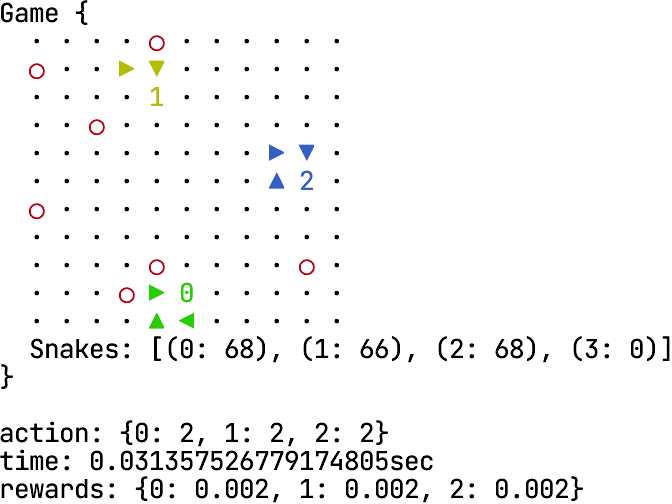
\includegraphics[width=0.4\linewidth]{vit_spin_render.png}
    \caption{Game rendering with the small ViT model spinning in a circle.
    }
    \label{fig:render}
\end{figure}

We tried to encourage exploration by adding an entropy bonus to the model.
However, after setting the entropy coefficient to 0.1,
our small ViT model could not learn to avoid walls even after training for
$32\times 16^4$ steps. Therefore,
we decided to lower the entropy coefficient to 0.01,
which resulted in our ViT model learning to spin again,
but reach for food when its health is low.
The deeper MLP model learned to spin after sufficient training,
no matter the entropy coefficient.

After we fixed the loading of previous models, added the food reward,
and increased the entropy coefficient to 0.1,
we trained the small ViT model for $587\times 16^4$ steps and the big ViT model
for $339\times 16^4$ steps (counting previous steps trained). However,
the small ViT model still has a less intense tendency to spin,
while neither models can avoid walls or themselves consistently.
We note that the major bottleneck in training is the training efficiency and
getting enough training steps for the model to converge.

We attempted to test the models against the tree search agent. However,
the tree search agent does not make simple mistakes like running into walls or
itself when it has a choice,
therefore the models can never win against the tree search agent in our
observation. We suspect this is why~\cite{chung2020battlesnake}
does not use standard agents as comparison and rather compare the models against
themselves. For the above reason,
we will not evaluate the models against the tree search agent,
but rather against other models.

\section{Final Report Plan}

\todo{The plan for finalizing your final report.}

To finalize our report, we plan to focus on continue training the small ViT model for more steps,
while investigating alternatives to allow the model to compete with other agents
on the leaderboard~\cite{standard_leaderboard}.
Since the training process is the major bottleneck,
and the models are still not performing well,
we have to reach for alternative approaches to improve the model's performance.
One such solution is to combine the model predictions with tree search,
such as the method applied in AlphaGo~\cite{silver2016mastering}.
We will use the policy probability outputs from the model to narrow down the
tree search options.

For evaluation,
we will develop a Battlesnake-protocol-compatible web server that implements the
above hybrid solution~\cite{battlesnake},
and test the model against other models on the leaderboard. With this approach,
we aim to test the model's performance in a real-world scenario and fulfill our
promise in this direction.

\printbibliography

\end{document}
